
\section{Interference of Light From Multiple Slits}
\label{interference_lab}
\makelabheader %(Space for student name, etc., defined in master.tex)

\textbf{Objective}

In this laboratory you will investigate the wave-like nature of light by measuring the interference 
between light beams produced by a laser shining through a set of narrow, adjacent
slits. 
%\begin{itemize}
%\item To investigate the interference of light waves as they pass through
%a set of slits. 
%\end{itemize}

\textbf{Apparatus}

\begin{itemize}
\item Basic optics diode laser
\item Optical bench with rotary motion sensor
\item Phototransistor for measuring light intensity (mounted on rotary motion sensor)
\item ``Multiple Slit Set'' slit accessory
%\item ``Single Slit Set'' slit accessory
\item Small plastic ruler
%\item Glass plate with sets of narrow slits
\item {\it DataStudio} 750 Interface
\end{itemize}

%\textbf{Introduction}

\textbf{Activity 1: An Alternative View of Light}

Isaac Newton believed that light was made up of small, unseen particles
that obeyed (surprisingly enough!) Newton's Laws. This view is known
as the corpuscular theory. Let's briefly consider how this model of light
predicts different behavior from the wave theory.

(a) Consider a laser beam shining on a circular hole. If a beam of
light consisted of small, unseen particles that behaved as tiny billiard
balls what would you see on a screen that is downstream from the circular
hole? A sketch might be useful here.  (This question and the next one aren't meant to be hard.
They're just getting at your common sense notions about how shadows work.)
\answerspace{35mm}

(b) Now consider the same laser beam shining on a pair of narrow slits.
What would you see on a screen downstream from the slits if light
were made of corpuscles?
\answerspace{35mm}

\pagebreak[2]
For the questions above you probably predicted that the laser would
form a single bright spot (for part a) or two parallel lines (for part
b).  In fact, the experiment you are about to perform challenges Newton's corpuscular theory. 
It turns out that when light passes through a set of narrow slits, each opening acts as an independent
source of waves that can overlap one another to produce a distinctive
pattern of bright and dark spots on a screen. 

\textbf{Activity 2: Measuring the Interference of Light }

You will measure this ``interference pattern'' with the setup shown below. 
(This is a \underline{top} view of the set-up.) 
A phototransistor detector is seated behind the narrow opening on top of the large,
metal mount sitting on a rail. The detector can convert the intensity 
of the light falling on it into a voltage signal that can be read by the
computer. In addition, the detector can be moved back and
forth on a rotary motion sensor that measures the detector's position. These two signals can be combined to
make a graph of the intensity as a function of position.

\answerspace{0.3cm}
{\centering \resizebox*{0.75\textwidth}{!}{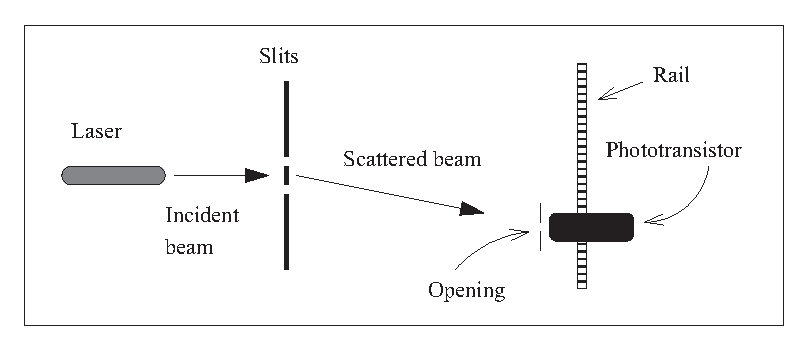
\includegraphics{interference_of_light/interference_of_light_fig1b_bw.eps}} \par}
\answerspace{0.3cm}

(a) Mount the laser on the 
optical bench at the opposite end from the rotary motion sensor.
DO NOT LOOK DIRECTLY INTO
THE BEAM OR POINT THE LASER CARELESSLY ABOUT THE ROOM.  Turn on the
laser.  You should see the bright red spot of the beam striking
the rotary motion assembly with the detector on it. 
Use the two adjustment screws on the back of the laser to to make the beam hit the exact center of the opening in front of the detector when it is positioned in the middle of its travel range.  

%\vspace{10mm}

(b) On the detector itself, set the small gain switch to ``100'' (highest sensitivity).  Rotate the aperture wheel in front of the detector to the position marked ``3''.  (Wider gaps let in more light; narrower gaps measure light at a more precisely defined location.)  Also check that the detector is exactly perpendicular to the incident beam; adjust its mounting if necessary.

%\vspace{10mm}

(c) Identify the ``Multiple Slit Set'' slit accessory.  You will place this on the optical bench near the laser, about 70 or 80 cm away from the detector.  Select a double slit of width .04 mm and separation .125 mm, marked by the number ``2''. You can rotate the wheel with the slits AND rotate where the slit wheel is mounted on the plastic frame.  
Rotate both so that when you click the frame onto the optical bench, the double slit that you want is at the center of the opening, with the slits oriented vertically and the laser beam centered right on it.  You should now see the ``interference pattern,'' consisting of a series of bright spots a few millimeters apart, on the white screen in front of your detector.

%\vspace{10mm}

(d) Start the ``Interference'' activity in the {\bf 132 Workshop} folder. 
When you are ready, click {\bf Start} and slowly move the detector 
from one side of the slide of the bright spots to the other by turning the wheel on the rotary 
motion sensor. Move carefully and take about 4-5 seconds to complete the 
motion. 
As you move it, the computer screen should show a graph of the intensity reading versus the position reading. 
Click {\bf Stop} when you're done. 
The graph, called the interference pattern, should be a symmetric pattern of distinct peaks. Consult your instructor if your setup isn't working.

\pagebreak[2]
(e) In the space below, draw a good graph showing your interference pattern.  
Be sure to label your axes!
\answerspace{1.5in}

\textit{(If your instructor requests it, make a hardcopy of this graph and attach it to this unit.)}

\textbf{What's Going On?}

Let's think about why your interference pattern looks the way it does.  When the laser hits the two slits, 
light comes out of the slits in all directions all at once, as in the diagram (a) below.  
But that's a lot of light rays to keep track of, so we'll focus on just two at a time, always in the same direction, as in (b) below.
We'll define $\theta$ as the angle of the rays, where $\theta=0$ means straight ahead.  

\vspace{-0.1in}
\begin{center}
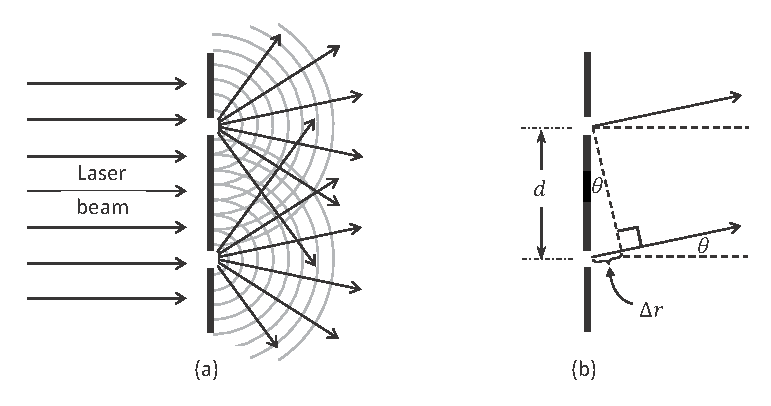
\includegraphics[width=0.63\textwidth]{interference_of_light/rays2.eps}
\end{center}
\vspace{-0.2in}

The pair of rays will converge at the same spot on the screen or at the detector.  (``Wait!  How can they converge if they're parallel?!?''  Okay, they're not \textit{perfectly} parallel, but they're pretty close.  After all, the two slits are only separated by a fraction of a millimeter, and the detector is almost a meter away.  The math is way easier if we approximate the rays as parallel.)
What makes the series of bright and dark areas on the screen or at the detector is that the rays travel slightly different distances to get there.  
The difference in path length is shown on the diagram above as $\Delta r$.  

(f) For a particular angle $\theta$, if the path difference $\Delta r$ happens to be an exact integer multiple of the light's wavelength $\lambda$, will the two waves combine \textit{CON-structively} or \textit{DE-structively}?  (And does that correspond to a bright spot or a dark spot?)
\answerspace{0.5in}

(g) For a particular angle $\theta$, if the path difference $\Delta r$ happens to be an exact half-integer multiple of the light's wavelength $\lambda$ (like $0.5\lambda$ or $3.5\lambda$), will the two waves combine \textit{CON-structively} or \textit{DE-structively}?
\answerspace{0.5in}

(h) What about if the path difference $\Delta r$ happens to be something in between, like $\Delta r = 2.3\lambda$, or $0.8\lambda$? Would that place on the screen be bright? Or dark? Or something in between?
\answerspace{0.5in}

\textit{Imagine slowly increasing $\theta$, starting from zero.   As the path difference $\Delta r$ increases, the interference between the two rays oscillates between constructive and destructive, causing the oscillating pattern on your graph.}

\pagebreak[2]
\textbf{Activity 3: Determining the Wavelength of the Laser }

Now you'll use the geometry of your setup to measure the actual wavelength $\lambda$ of the light from your laser!

(a) Looking at your graph, the highest maximum is straight ahead of the slits ($\theta=0$), where $\Delta r=0$.  Does the next maximum to the right of that correspond to $\Delta r=2\lambda$?  Or $3\lambda$?  Or $19\lambda$?  Or something else?

\vspace{0.1in}
\hspace{0.8in}$\Delta r=$
\vspace{0.1in}

(b) Are the two $\theta$'s in the drawing on the last page the same?
\answerspace{0.3in}

(c) Write $\Delta r$ in terms of the distance between the slits $d$ and the the angle $\theta$.
\answerspace{0.5in}

(d) Write $\theta$ in terms of the length $L$ between the detector and the slits and the horizontal distance $\Delta x$ between the central maximum and the next maximum to the right of it..
\answerspace{0.5in}

(e) Measure $L$ carefully, using a straight edge to align objects to the scale on your tracks.  (The phototransistor detector is actually 25 mm behind the aperture.)  For measuring $\Delta x$ the ``Smart Tool'' on DataStudio isn't actually that smart, and won't give you enough significant digits; just read the positions of the peaks carefully from the graph, expanding the scales by dragging them if you need to.  What are your values for $L$, $\Delta x$, and $\theta$?
\answerspace{0.8in}

(f) Combine your answers for parts (a) through (e) to calculate a value for $\lambda$.  
\answerspace{1in}

(g) Does your value correspond to an accepted value for red light?
\answerspace{0.3in}

You just found that the \textit{first} maximum to the right of the center happens at an angle $\theta$ where $d \sin \theta = \lambda$.  Other maxima occur wherever $\Delta r$ is any other integer multiple of $\lambda$, so in general there are intensity maxima at any $\theta$ where
\begin{displaymath}
d \sin \theta = m \lambda,
\end{displaymath}
where $m$ is some integer 0, 1, 2, 3, and so on.  

(h) Try calculating the wavelength of the laser light again, this time using the locations of the central maximum ($m=0$) and the one for $m=3$.  (If $m=3$ is hard to see, $m=2$ is okay too.)
\answerspace{1.0in}


\pagebreak[2]
\textbf{Activity 4: More Than Two Slits}

(a) What if, instead of two slits, you shined the laser on a series of three or four slits, all equally spaced?  Would you still see an interference pattern?  Would the spacing between maxima be the same?  What is your prediction?
\answerspace{0.8in}

(b) To look for any differences, you will want to have the smoothest, nicest interference pattern you can get.  If your data for the two-slit interference pattern isn't \textit{really} pretty, measure it again.  

(c) Now, without deleting your previous data, switch to three slits by rotating the wheel on the slit accessory 
to ``3'', and run the pattern again.  (After hitting \textbf{stop}, you may want to hit the
``\raisebox{-1mm}{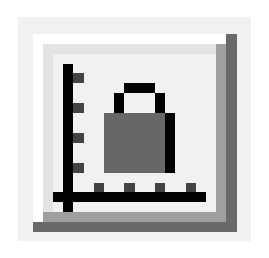
\includegraphics[width=5mm]{interference_of_light/icon_bw.eps}}''
button to ``lock the graphs'' together with the same scale axes.  Then hit the icon again to unlock the graphs, allowing you to align the peaks horizontally with each other.)  What about the interference pattern has changed, and what has stayed the same?
\answerspace{0.8in}

(d) What happens with four slits?  Or five slits?
\answerspace{0.8in}

(e) Suppose we have three slits all a distance $d$ apart, and we draw three parallel rays from them, 1, 2, and 3.  For an angle $\theta$ at which the path difference between rays 1 and 2 just happens to be $\Delta r_{12} = \lambda$, what is the path difference $\Delta r_{13}$ between rays 1 and 3?  (A good picture might help....)
\answerspace{1.5in}

(f) Is there any angle $\theta$ at which rays 1 and 2 interfere perfectly constructively with each other,  but ray 3 interferes destructively with either of them?
\answerspace{0.4in}

\pagebreak[2]
(g) Suppose you have five rays, 1, 2, 3, 4, and 5, and suppose we consider an angle $\theta$ at which the path difference between the first two is $\Delta r_{12} = 0.8\lambda$.  What are the distances $\Delta r_{13}$, $\Delta r_{14}$, and $\Delta r_{15}$?  (Again, a good picture would help.)
\answerspace{2.5in}

(h) In the case in (g), would rays 1 and 3 interfere \textit{CON-structively} or \textit{DE-structively}?  What about rays 1 and 4?
\answerspace{0.8in}

(i) If you combined all five rays together, would the result at the detector be a place of high intensity or low intensity? 
\answerspace{0.6in}

(j) If there were only TWO slits, and you combined only TWO rays together with a path difference of $\Delta r_{12} = 0.8\lambda$, would the result at the detector be a place of high intensity or low intensity? 
\answerspace{0.6in}

(k) In general, as you increase the number of slits, do the maxima in the interference pattern become broader or narrower?  Does the maximum intensity increase or decrease?
\answerspace{0.6in}

\textbf{Activity 5: One More Thing...}

Remember the earlier discussion in Activity 1 of Newton's corpuscular theory of
light? You've taken a ton of data by now.  Does your data support Newton's theory or the wave theory of light?
Explain.
\answerspace{1.0in}
